\documentclass{article}

\usepackage[left=1in, top=1in, right=1in, bottom=1in]{geometry}
\usepackage{graphicx, color}
\usepackage{url}
\usepackage[linesnumbered,ruled,vlined]{algorithm2e}
\usepackage{framed}
\usepackage{here}
\usepackage{zi4}
\usepackage{color}
\usepackage{Sweave}
\renewcommand{\baselinestretch}{1.2}

% \VignetteIndexEntry{glmnetLRC Example}

\begin{document} 
\Sconcordance{concordance:glmnetLRC.tex:/Users/d3p423/Work/github/glmnetLRC/vignettes/glmnetLRC.Rnw:%
1 54 1 1 3 2 0 1 3 1 0 1 3 14 0 1 4 5 0 1 2 7 1 1 4 3 0 1 2 6 0 1 2 4 1 %
1 5 4 0 1 3 9 0 1 2 16 1 1 3 2 0 1 6 8 0 1 3 6 1 1 2 9 0 1 2 3 1 1 2 12 %
0 1 2 12 1 1 3 2 0 1 4 14 0 1 2 4 1 1 3 13 0 1 2 1 3 2 0 1 3 8 0 1 3 1 %
0 1 3 12 0 1 3 12 0 1 2 1 1 1 2 9 0 1 2 13 1 1 2 5 0 1 2 176 1}


\title{{\tt glmnetLRC}: Generalized Elastic Net Logistic Regression \\}
\author{Alex Venzin, Landon Sego}
\maketitle

The {\tt glmnetLRC} package extends the {\tt glmnet} package by making it possible to train elastic net logistic regression models using a customized discrete loss function.  This allows users to assign unique loss values to false positive and false negative errors. This approach was originally implemented to automate the process of determining the curation quality of mass spectrometry samples. Some of the data documented in \cite{thepaper} will be used here to demonstrate how to train your own classifier. The elastic net parameter estimates are obtained by maximizing a penalized likekihood function. The penalty is essentially a weighted average of the ridge penalty ($\ell_2$ norm) and the lasso penalty ($\ell_1$ norm) of the regression parameters.  This approach balances feature selection and model simplicity. 
Let's begin by loading the package and the training data:
\begin{Schunk}
\begin{Sinput}
> # Load the package
> require(glmnetLRC)
> # Load the VOrbitrap Shewanella QC data
> data(traindata)
> # A view of first five rows and columns
> traindata[1:5, 1:5]
\end{Sinput}
\begin{Soutput}
      Instrument_Category Instrument Dataset_ID Acq_Time_Start Acq_Length
pt701           VOrbitrap VOrbiETD03     251690     12/31/2011         98
pt702           VOrbitrap VOrbiETD03     251706       1/1/2012         98
pt703           VOrbitrap VOrbiETD03     251887       1/4/2012         98
pt704           VOrbitrap VOrbiETD03     252361      1/10/2012         98
pt705           VOrbitrap VOrbiETD04     255284       2/2/2012         99
\end{Soutput}
\begin{Sinput}
> # Here we select the predictor variables
> predictors <- as.matrix(traindata[,9:96])
\end{Sinput}
\end{Schunk}

\noindent {\tt glmnetLRC} requires a binary response variable, coded
as class {\tt factor} in {\tt R}.  The order in which the response variable
is coded is important.  Specifically, the class we want to predict with
the greatest sensitivity should be encoded as the second level. To illustrate how this
is done, consider the Shewanella QC data, where the objective is to be
sensitive to predicting poor datasets.  Hence we 
code ``poor" last, as follows:
\begin{Schunk}
\begin{Sinput}
> response <- factor(traindata$Curated_Quality,
+                    levels = c("good", "poor"),
+                    labels = c("good", "poor"))
\end{Sinput}
\end{Schunk}
\noindent Now we must define a discrete loss matrix. For the curation
of dataset quality, predicting ``good" when the dataset is ``poor" is considerably 
worse (Loss = 5) than predicting ``poor" when the dataset
is ``good" (Loss = 1).  Correct predictions receive a penalty of zero loss:

\begin{Schunk}
\begin{Sinput}
> lM <- lossMatrix(c("good","good","poor","poor"),
+                  c("good","poor","good","poor"),
+                  c(     0,     1,     5,     0))
> # Observe the structure of the loss matrix
> lM
\end{Sinput}
\begin{Soutput}
           Predicted.good Predicted.poor
Truth.good              0              1
Truth.poor              5              0
\end{Soutput}
\end{Schunk}

To train the elastic net model, the user needs to supply a handful of arguments to the {\tt glmnetLRC} function. The mandatory arguments are the true class labels, {\tt truthLabels} (which, for training, is the response variable), the set of predictor variables, {\tt predictors} (as a matrix or dataframe),
and the loss matrix {\tt lossMat}. Noteworthy additional arguments include {\tt tauVec}, a vector of potential thresholds $\tau \in (0, 1)$ that are used to dichotomize the predicted probabilities from the logistic regression into two class labels; {\tt alphaVec}, a vector of potential values of the elastic net mixing parameter $\alpha \in [0, 1]$; {\tt cvFolds}, the number of cross validation folds; and {\tt seed}, the random number seed for partitioning the data into the cross validation folds. Keep in mind that $\alpha$ governs the tradeoff between the two regularization penalties. When $\alpha = 0$, the objective is $\ell_2$ regularization (ridge regression) and when $\alpha = 1$, the objective is $\ell_1$ regularization (lasso regression).   

Be advised that heavier sampling of {\tt tauVec} or {\tt alphaVec} (i.e., sequences of greater length) leads to increased computation time, but more of the parameter space will be sampled, potentially leading to a better classifier. To get a step by step elicitation of the algorithm that generates the classifier, refer to the appendix.  We now train the elastic net logistic regression using the default settings for $\tau$ and the number of cross validation
folds (which is 5) and restricting $\alpha = (0.5, 1)$:
\begin{Schunk}
\begin{Sinput}
> ncores <- max(1, detectCores() - 1)
> glmnetLRC_fit <- glmnetLRC(response, predictors, lM, cores = ncores,
+                             alphaVec = c(1, 0.5), tauVec = c(0.3, 0.5, 0.7),
+                             cvReps = ncores)
> 
\end{Sinput}
\end{Schunk}

\noindent The call to {\tt glmnetLRC} uses cross validation to solve for the optimal parameter settings $\left(\alpha, \lambda, \tau\right)$ that minimize the expected loss for the elastic net logistic regression model. Printing the resulting object shows the median value for the parameters over {\tt cvReps}.
 
\begin{Schunk}
\begin{Sinput}
> print(glmnetLRC_fit)
\end{Sinput}
\begin{Soutput}
The optimal parameter values for the elastic net logistic regression fit: 
     Df      %Dev alpha     lambda tau
[1,]  7 0.6488163     1 0.03921906 0.3
\end{Soutput}
\end{Schunk}
 
Now that the classifier has been properly trained and the optimal parameters have been identified, we are interested in making predictions for new data observations. This requires the elastic net regression model (the output from {\tt glmnetLRC}) and the set of new observations to be predicted, {\tt newdata}.  If true labels are available in {\tt newdata}, the column containing these true class labels can be specified via {\tt truthCol}. Additionally, one may wish to carry through a subset of the explanatory variables in {\tt newdata}.  These columns are indicated using {\tt keepCols}.   True labels are not required to make predictions---but they are required to compute performance metrics (sensitivity, specificity, etc.) for the elastic net logistic regression model. We begin by testing the classifer on the training data:
\begin{Schunk}
\begin{Sinput}
> predictTrain <- predict(glmnetLRC_fit, traindata, truthCol = "Curated_Quality", keepCols = 1:2)
> # Look at beginning of the predicted data.  Note the extra columns that were kept.
> head(predictTrain)
\end{Sinput}
\begin{Soutput}
      PredictClass Curated_Quality Instrument_Category Instrument
pt701         good            good           VOrbitrap VOrbiETD03
pt702         good            good           VOrbitrap VOrbiETD03
pt703         good            good           VOrbitrap VOrbiETD03
pt704         poor            good           VOrbitrap VOrbiETD03
pt705         good            good           VOrbitrap VOrbiETD04
pt706         poor            poor           VOrbitrap VOrbiETD02
\end{Soutput}
\begin{Sinput}
> # Summarize the peformance of the new classifier in terms of a 
> # variety of metrics:
> summary(predictTrain)
\end{Sinput}
\begin{Soutput}
                          poor
sensitivity         0.90000000
specificity         0.90855457
false negative rate 0.10000000
false positive rate 0.09144543
accuracy            0.90631808
\end{Soutput}
\end{Schunk}
\noindent Note how the sensitivity for detecting poor datsets is considerably better than the specificity.  That reflects the loss function that penalizes incorrectly classifying a poor dataset more severely than misclassifying a good dataset.

\noindent Now let's bring in some new data and examine the performance of the classifier:
\begin{Schunk}
\begin{Sinput}
> # load the data for testing
> data(testdata)
> # Create table observing the true number of good/poor items 
> with(testdata, table(Curated_Quality))
\end{Sinput}
\begin{Soutput}
Curated_Quality
good poor 
  38   62 
\end{Soutput}
\begin{Sinput}
> # Predict new data
> predictTest <- predict(glmnetLRC_fit,testdata,
+                        truthCol = "Curated_Quality")
> # Look at the first few rows
> head(predictTest)
\end{Sinput}
\begin{Soutput}
     PredictClass Curated_Quality
931          poor            good
1449         good            good
1467         good            good
1468         good            good
1470         good            good
1501         good            good
\end{Soutput}
\begin{Sinput}
> # Summarize the output of predicting the data we trained on 
> summary(predictTest)
\end{Sinput}
\begin{Soutput}
                          poor
sensitivity         0.91935484
specificity         0.89473684
false negative rate 0.08064516
false positive rate 0.10526316
accuracy            0.91000000
\end{Soutput}
\end{Schunk}

\noindent Finally, we would like to get a sense of the distribution of the parameters that were chosen during the cross validation phase. The {\tt plot} method produces a 3 x 3 scatterplot matrix of the optimal triples $(\alpha, \lambda, \tau)$ associated with the selected regression model from each cross validation replicate. The univariate distribution of each parameter is plotted on the diagonal of the scatterplot matrix.

\begin{figure}[H]
\begin{center}
\begin{Schunk}
\begin{Sinput}
> plot(glmnetLRC_fit)
\end{Sinput}
\end{Schunk}
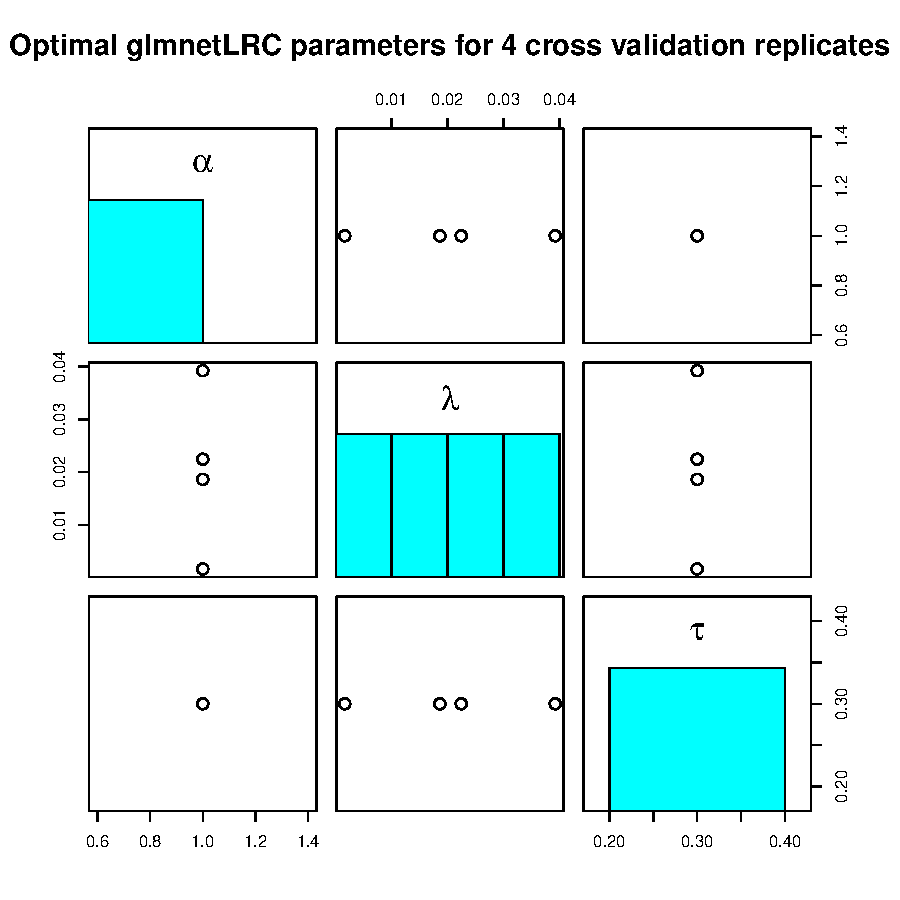
\includegraphics{glmnetLRC-plot}
\caption{Scatterplot matrix of optimization parameters}
\end{center}
\end{figure}

\appendix

Presented below is a high-level explanation of the parameter selection algorithm.

\begin{algorithm} \label{glmnetLRC}

\KwIn{$truthLabels$ = Labels associated with binary outcome, 
      $predictors$ = matrix of explanatory variables,
      $lossMat$ = user defined discrete loss matrix,
      $weight$ = vector of weights to fit elastic net model,
      $\alpha$ = vector of elastic net missing parameters,
      $\tau$ = vector of $\tau$ values,
      $cvFolds$ = cross-validation folds,
      $seed$ = random number seed}
      
\KwOut{$parameters$ = $(\alpha, \lambda, \tau)$ triple that minimizes
expected loss, $(\tau - 0.5)^{2}$, and $\lambda$}

// For each unique combination of $\alpha$ and {\tt cvFolds}, generate a $\lambda$ 
// sequence using {\tt glmnet}, fit an elastic net logisitc regression model, predict 
// on validation set, and calculate the loss

$ \textrm{Loss} \gets array() $\;
$ \textrm{params} \gets array() $\;
\For{$a \in \alpha$} {
  \For{$ v \in cvFolds$} {
  
    $\lambda \gets glmnet(predictors, truthLabels, weight, a)\$\lambda $\;
    $\textrm{model} \gets glmnet(predictors, truthLabels, weight, a, \lambda) $\;
    $\textrm{LossCalc} \gets predict.loss(model, lossMat, \tau, a, \lambda,
    predictors, truthLabels, weight) $\;
    $\textrm{params} \gets array(a, \lambda, \tau, model, LossCalc) $\;
    
  }
  
  $ Loss[ \alpha ] \gets params $\; 
  
}

// Calculate expected loss over all training folds \; 

$\textrm{out} \gets array() $\;

\For{$v \in cvFolds$}{
  $Eloss \gets \frac{params[LossCalc[v]]}{\sum weight[v]} $\;
  $out[v] \gets array(Eloss, params[\alpha [v]], params[\lambda [v]], params[\tau [v]], seed) $\; 
}

// sort the output based on objective $\textrm{min} Eloss + (\tau - 0.5)^{2} - \lambda$

$sorted.out \gets sort(out, by = Eloss + (\tau - 0.5)^{2} - \lambda) $\;

// optimal parameters will be first row entry
	
\Return{$parameters = sorted.out[1,]$}
\caption{{\sc glmnetLRC} searches the parameter space of $(\alpha, \lambda, \tau)$ for the 
combination that minimizes expected loss with respect to the user specified loss matrix.}
\end{algorithm}  


\nocite{*}
\bibliography{glmnetLRC}
\bibliographystyle{plain}	

\end{document}
